\documentclass{article}
\usepackage{graphicx}
\usepackage{threeparttable}
\usepackage{float}
\usepackage{textcomp}
\usepackage[margin=1in]{geometry}

\begin{document}

\section{FEW}

\begin{table}[H]
    \centering
    \caption{H5--H11: BC vs. named-scenario contrasts.}
    \begin{tabular}{ l c c c }
\hline \hline
contrast & estimate & se & N \\
\hline
\hspace{0.05cm} BC vs BI & 0.625** & (0.042) &  76 \\
\hspace{0.05cm} BC vs BG & 0.600** & (0.042) &  85 \\
\hspace{0.05cm} BC vs BN & 0.500 & (0.042) &  83 \\
\hspace{0.05cm} BC vs BC\_SD & 0.559 & (0.040) & 102 \\
\hspace{0.05cm} BC vs BCmat & 0.491 & (0.040) & 107 \\
\hspace{0.05cm} BC vs BCflight & 0.715$^\dagger$ & (0.040) &  86 \\
\hspace{0.05cm} BC vs BCbeef & 0.536 & (0.042) &  97 \\
\hline
\hspace{0.05cm} R-squared & \multicolumn{3}{c}{0} \\
\hline \hline
\end{tabular}
\begin{tablenotes}
\small
\item \textit{Notes:} Estimate = share choosing BC (HC1-robust SE in parentheses). *** p$<$0.01, ** p$<$0.05, * p$<$0.1 (FDR-adjusted). One-sided test direction per pre-registration: H5--H9 (BI/BG/BN/BC\_SD/BCmat) test H1: share $>$ 0.5 (BC preferred); H10--H11 (BCflight/BCbeef) test H1: share $<$ 0.5 (the alternative scenario is preferred). $^\dagger$ = significant (two-sided, unadjusted p$<$0.1) in the direction OPPOSITE the pre-registered hypothesis - a real effect, just not the one predicted. R2 is 0 by construction (intercept-only models).
\end{tablenotes}
    \label{tab:table1}
\end{table}


\begin{table}[H]
    \centering
    \caption{Bradley--Terry ranking of the 12 named scenarios.}
    \begin{tabular}{ l c c c }
\hline \hline
scenario & ability & se & N \\
\hline
\hspace{0.05cm} BC & ref. &  & 720 \\
\hspace{0.05cm} BN & -0.027 & (0.127) & 356 \\
\hspace{0.05cm} BCmat & -0.126 & (0.118) & 416 \\
\hspace{0.05cm} BC45k & -0.233* & (0.122) & 379 \\
\hspace{0.05cm} BG & -0.264** & (0.122) & 388 \\
\hspace{0.05cm} BC90k & -0.350*** & (0.120) & 404 \\
\hspace{0.05cm} BCbeef & -0.443*** & (0.122) & 374 \\
\hspace{0.05cm} BCflight & -0.538*** & (0.128) & 334 \\
\hspace{0.05cm} BI & -0.585*** & (0.132) & 319 \\
\hspace{0.05cm} BC\_SD & -0.615*** & (0.122) & 389 \\
\hspace{0.05cm} BC120k & -0.725*** & (0.124) & 376 \\
\hspace{0.05cm} BI120k & -0.999*** & (0.126) & 393 \\
\hline
\hspace{0.05cm} R-squared & \multicolumn{3}{c}{0.034} \\
\hline \hline
\end{tabular}
\begin{tablenotes}
\small
\item \textit{Notes:} Ability = log-strength relative to BC (reference, fixed at 0); SE in parentheses. *** p$<$0.01, ** p$<$0.05, * p$<$0.1 (FDR-adjusted Wald test vs. BC). R2 = McFadden pseudo-R2. "I don't know" pairs excluded (Bradley-Terry requires a discrete winner); contrast with the other tables, where they are kept as indifference (selected = 0.5).
\end{tablenotes}
    \label{tab:table2}
\end{table}


\section{ANY}

\begin{table}[H]
    \centering
    \caption{H1--H4: primary specification results.}
    \begin{tabular}{ l c c }
\hline \hline
 & estimate & se \\
\hline
\hspace{0.05cm} Temperature & -0.054*** & (0.005) \\
\hspace{0.05cm} Income (per 1k/month) & -7.85e-07 & (1.65e-05) \\
\hspace{0.05cm} Working hours & F = 6.358*** &  \\
\hspace{0.05cm} \hspace{1em} 32h/week (vs. 40h) & -0.043 & (0.027) \\
\hspace{0.05cm} \hspace{1em} 36h/week (vs. 40h) & 0.009 & (0.016) \\
\hspace{0.05cm} \hspace{1em} 44h/week (vs. 40h) & -0.007 & (0.015) \\
\hspace{0.05cm} Public services: increased (vs. stable) & 0.028*** & (0.008) \\
\hspace{0.05cm} Beef \& flights restrictions & F = 0.687 &  \\
\hspace{0.05cm} \hspace{1em} Less beef (vs. stable) & -0.015 & (0.011) \\
\hspace{0.05cm} \hspace{1em} Less flights (vs. stable) & -0.011 & (0.011) \\
\hspace{0.05cm} \hspace{1em} Less beef \& flights (vs. stable) & -0.010 & (0.011) \\
\hspace{0.05cm} National redistribution (vs. current) & 0.027*** & (0.007) \\
\hspace{0.05cm} Global redistribution (vs. current) & 0.014* & (0.008) \\
\hspace{0.05cm} Working hours $\times$ growth & -0.003** & (0.001) \\
\hspace{0.05cm} Future income $>$ current & 0.014 & (0.013) \\
\hline
\hspace{0.05cm} Observations & \multicolumn{2}{c}{3,247} \\
\hspace{0.05cm} R-squared & \multicolumn{2}{c}{0.021} \\
\hline \hline
\end{tabular}
\begin{tablenotes}
\small
\item \textit{Notes:} Cluster-robust (respondent-level) SE in parentheses. *** p$<$0.01, ** p$<$0.05, * p$<$0.1. Main-attribute and hypothesis rows: FDR-adjusted (10-test pre-registered family; the one-sided Temperature test is part of this family but not shown as its own row, since it duplicates the two-sided Temperature row above). Indented individual dummy-level rows: descriptive detail, unadjusted p-values.
\end{tablenotes}
    \label{tab:table3}
\end{table}


\begin{table}[H]
    \centering
    \caption{H1--H4 robustness check: excluding income $>$ P99.}
    \begin{tabular}{ l c c }
\hline \hline
 & estimate & se \\
\hline
\hspace{0.05cm} Temperature & -0.053*** & (0.005) \\
\hspace{0.05cm} Income (per 1k/month) & -1.84e-04 & (5.53e-04) \\
\hspace{0.05cm} Working hours & F = 9.185*** &  \\
\hspace{0.05cm} \hspace{1em} 32h/week (vs. 40h) & -0.052* & (0.028) \\
\hspace{0.05cm} \hspace{1em} 36h/week (vs. 40h) & 0.009 & (0.016) \\
\hspace{0.05cm} \hspace{1em} 44h/week (vs. 40h) & -0.010 & (0.015) \\
\hspace{0.05cm} Public services: increased (vs. stable) & 0.025*** & (0.008) \\
\hspace{0.05cm} Beef \& flights restrictions & F = 0.986 &  \\
\hspace{0.05cm} \hspace{1em} Less beef (vs. none) & -0.017* & (0.010) \\
\hspace{0.05cm} \hspace{1em} Less flights (vs. none) & -0.011 & (0.010) \\
\hspace{0.05cm} \hspace{1em} Less beef \& flights (vs. none) & -0.012 & (0.011) \\
\hspace{0.05cm} National redistribution (vs. current) & 0.027*** & (0.007) \\
\hspace{0.05cm} Global redistribution (vs. current) & 0.019** & (0.007) \\
\hspace{0.05cm} Working hours $\times$ growth & -0.003** & (0.001) \\
\hspace{0.05cm} Future income $>$ current & 0.007 & (0.015) \\
\hline
\hspace{0.05cm} Observations & \multicolumn{2}{c}{3,464} \\
\hspace{0.05cm} R-squared & \multicolumn{2}{c}{0.021} \\
\hline \hline
\end{tabular}
\begin{tablenotes}
\small
\item \textit{Notes:} Primary specification re-estimated excluding respondents whose declared current income, annualized and adjusted for household size, exceeds the 99th percentile of the (2025) Italian income distribution (91 respondent(s) excluded; threshold = 134640 EUR/year per adult). Same specification, columns and stars convention as the primary H1--H4 table - compare directly to check sensitivity to this exclusion.
\end{tablenotes}
    \label{tab:table4}
\end{table}


\input{table5.tex}

\begin{table}[H]
    \centering
    \caption{Secondary specification search: top 15 candidates.}
    \begin{tabular}{ l c c c c c }
\hline \hline
Rank & Income & Temperature & Hours & Extra interaction & Adj. R2 \\
\hline
\hspace{0.05cm}  1 & threshold & pairwise\_binary & categorical & none & 0.0200 \\
\hspace{0.05cm}  2 & threshold & pairwise\_binary & categorical & growth\_x\_income & 0.0199 \\
\hspace{0.05cm}  3 & threshold & linear & categorical & none & 0.0197 \\
\hspace{0.05cm}  4 & threshold & quadratic & categorical & none & 0.0196 \\
\hspace{0.05cm}  5 & threshold & pairwise\_binary & quadratic & none & 0.0196 \\
\hspace{0.05cm}  6 & threshold & linear & categorical & growth\_x\_income & 0.0196 \\
\hspace{0.05cm}  7 & threshold & pairwise\_binary & pairwise\_binary & none & 0.0196 \\
\hspace{0.05cm}  8 & threshold & quadratic & categorical & growth\_x\_income & 0.0196 \\
\hspace{0.05cm}  9 & threshold & pairwise\_binary & quadratic & growth\_x\_income & 0.0196 \\
\hspace{0.05cm} 10 & threshold & pairwise\_binary & pairwise\_binary & growth\_x\_income & 0.0195 \\
\hspace{0.05cm} 11 & threshold & linear & quadratic & none & 0.0195 \\
\hspace{0.05cm} 12 & threshold & quadratic & quadratic & none & 0.0194 \\
\hspace{0.05cm} 13 & threshold & linear & quadratic & growth\_x\_income & 0.0194 \\
\hspace{0.05cm} 14 & excluded & pairwise\_binary & categorical & none & 0.0194 \\
\hspace{0.05cm} 15 & threshold & quadratic & quadratic & growth\_x\_income & 0.0194 \\
\hline \hline
\end{tabular}
\begin{tablenotes}
\small
\item \textit{Notes:} Out of 180 candidate specifications, ranked by adjusted R\textsuperscript{2}. Q5 grid: income inclusion/functional form, temperature/hours functional form, extra growth$\times$income interaction. Rank 1 is the winning specification reported in Table~\ref{tab:table5}.
\end{tablenotes}
    \label{tab:table6}
\end{table}


\begin{table}[H]
    \centering
    \caption{Primary specification with Elastic Net interactions.}
    \begin{tabular}{ l c c }
\hline \hline
 & estimate & se \\
\hline
\hspace{0.05cm} Temperature & -0.053*** & (0.005) \\
\hspace{0.05cm} Income (per 1k/month) & 0.000 & (0.000) \\
\hspace{0.05cm} Working hours: 32h (vs. 40h) & -0.042 & (0.026) \\
\hspace{0.05cm} Working hours: 36h (vs. 40h) & 0.015 & (0.015) \\
\hspace{0.05cm} Working hours: 44h (vs. 40h) & -0.009 & (0.015) \\
\hspace{0.05cm} Public services: increased (vs. stable) & 0.027*** & (0.007) \\
\hspace{0.05cm} Less beef (vs. none) & -0.013 & (0.010) \\
\hspace{0.05cm} Less flights (vs. none) & -0.009 & (0.010) \\
\hspace{0.05cm} Less beef \& flights (vs. none) & -0.007 & (0.010) \\
\hspace{0.05cm} National redistribution (vs. current) & 0.024*** & (0.007) \\
\hspace{0.05cm} Global redistribution (vs. current) & 0.018** & (0.007) \\
\hspace{0.05cm} 3\% productivity growth (vs. 1.5\%) & 0.128* & (0.067) \\
\hspace{0.05cm} Working hours $\times$ growth & -0.002** & (0.001) \\
\hspace{0.05cm} Future income $>$ current & 0.013 & (0.013) \\
\hline
\hspace{0.05cm} Observations & \multicolumn{2}{c}{3,555} \\
\hspace{0.05cm} R-squared & \multicolumn{2}{c}{0.02} \\
\hline \hline
\end{tabular}
\begin{tablenotes}
\small
\item \textit{Notes:} 0 interaction term(s) selected via Elastic Net added to the base specification. $\alpha$=0.5, main effects unpenalized, lambda.1se. Cluster-robust (respondent-level) SE in parentheses. *** p$<$0.01, ** p$<$0.05, * p$<$0.1 (unadjusted; descriptive, not part of the FDR-corrected pre-registered family). Compare to Table~\ref{tab:table3} (without these interactions).
\end{tablenotes}
    \label{tab:table7}
\end{table}


\begin{table}[H]
    \centering
    \caption{Secondary specification with Elastic Net interactions.}
    \begin{tabular}{ l c c }
\hline \hline
 & estimate & se \\
\hline
\hspace{0.05cm} Public services: increased (vs. stable) & 0.031*** & (0.008) \\
\hspace{0.05cm} Less beef (vs. none) & -0.010 & (0.010) \\
\hspace{0.05cm} Less flights (vs. none) & -0.006 & (0.010) \\
\hspace{0.05cm} Less beef \& flights (vs. none) & 0.001 & (0.010) \\
\hspace{0.05cm} National redistribution (vs. current) & 0.024*** & (0.007) \\
\hspace{0.05cm} Global redistribution (vs. current) & 0.017** & (0.007) \\
\hspace{0.05cm} 3\% productivity growth (vs. 1.5\%) & 0.110* & (0.066) \\
\hspace{0.05cm} Working hours $\times$ growth & -0.002* & (0.001) \\
\hspace{0.05cm} Temperature: 2.5\textendash{}3.5\textdegree C (vs. 1.7\textendash{}2.5\textdegree C) & -0.047*** & (0.009) \\
\hspace{0.05cm} Temperature: 3.5\textendash{}4.9\textdegree C (vs. 1.7\textendash{}2.5\textdegree C) & -0.110*** & (0.010) \\
\hspace{0.05cm} Working hours: 32h (vs. 40h) & -0.024 & (0.026) \\
\hspace{0.05cm} Working hours: 36h (vs. 40h) & 0.021 & (0.016) \\
\hspace{0.05cm} Working hours: 44h (vs. 40h) & -0.006 & (0.015) \\
\hspace{0.05cm} Income $>$ current & -0.001 & (0.015) \\
\hspace{0.05cm} Income $>$ 1.1$\times$ current & -0.006 & (0.011) \\
\hspace{0.05cm} Income $<$ 0.9$\times$ current & -0.060*** & (0.018) \\
\hline
\hspace{0.05cm} Observations & \multicolumn{2}{c}{3,555} \\
\hspace{0.05cm} R-squared & \multicolumn{2}{c}{0.021} \\
\hline \hline
\end{tabular}
\begin{tablenotes}
\small
\item \textit{Notes:} The same 0 Elastic-Net-selected interaction term(s) added to the secondary (highest adjusted R\textsuperscript{2}) specification. Cluster-robust (respondent-level) SE in parentheses. *** p$<$0.01, ** p$<$0.05, * p$<$0.1 (unadjusted; descriptive). Compare to Table~\ref{tab:table5} (without these interactions).
\end{tablenotes}
    \label{tab:table8}
\end{table}


\begin{table}[H]
    \centering
    \caption{Heterogeneity: primary specification.}
    \begin{tabular}{ l c c c }
\hline \hline
Attribute & Level & estimate & se \\
\hline
\multicolumn{4}{l}{\textbf{Age}} \\
\hspace{0.05cm} Temperature & 35-54 & 0.038** & (0.015) \\
\hspace{0.05cm} Temperature & 55+ & 0.023 & (0.015) \\
\hspace{0.05cm} Income (per 1k/month) & 35-54 & 0.001*** & (0.000) \\
\hspace{0.05cm} Income (per 1k/month) & 55+ & 0.000*** & (0.000) \\
\hspace{0.05cm} Working hours: 32h (vs. 40h) & 35-54 & -0.010 & (0.032) \\
\hspace{0.05cm} Working hours: 36h (vs. 40h) & 35-54 & -0.011 & (0.034) \\
\hspace{0.05cm} Working hours: 44h (vs. 40h) & 35-54 & -0.020 & (0.031) \\
\hspace{0.05cm} Working hours: 32h (vs. 40h) & 55+ & 0.024 & (0.032) \\
\hspace{0.05cm} Working hours: 36h (vs. 40h) & 55+ & 0.002 & (0.035) \\
\hspace{0.05cm} Working hours: 44h (vs. 40h) & 55+ & -0.002 & (0.032) \\
\hspace{0.05cm} Public services: increased (vs. stable) & 35-54 & 0.007 & (0.024) \\
\hspace{0.05cm} Public services: increased (vs. stable) & 55+ & 0.025 & (0.024) \\
\hspace{0.05cm} Less beef (vs. none) & 35-54 & -0.035 & (0.032) \\
\hspace{0.05cm} Less flights (vs. none) & 35-54 & 0.018 & (0.030) \\
\hspace{0.05cm} Less beef \& flights (vs. none) & 35-54 & -0.020 & (0.033) \\
\hspace{0.05cm} Less beef (vs. none) & 55+ & -0.028 & (0.032) \\
\hspace{0.05cm} Less flights (vs. none) & 55+ & 0.022 & (0.031) \\
\hspace{0.05cm} Less beef \& flights (vs. none) & 55+ & -0.012 & (0.034) \\
\hspace{0.05cm} National redistribution (vs. current) & 35-54 & -0.027 & (0.022) \\
\hspace{0.05cm} National redistribution (vs. current) & 55+ & -0.006 & (0.022) \\
\hspace{0.05cm} Global redistribution (vs. current) & 35-54 & 0.008 & (0.022) \\
\hspace{0.05cm} Global redistribution (vs. current) & 55+ & 0.007 & (0.022) \\
\hline
\multicolumn{4}{l}{\textbf{Gender}} \\
\hspace{0.05cm} Temperature & Male & 0.006 & (0.010) \\
\hspace{0.05cm} Income (per 1k/month) & Male & -0.000* & (0.000) \\
\hspace{0.05cm} Working hours: 32h (vs. 40h) & Male & -0.007 & (0.021) \\
\hspace{0.05cm} Working hours: 36h (vs. 40h) & Male & -0.010 & (0.021) \\
\hspace{0.05cm} Working hours: 44h (vs. 40h) & Male & 0.041** & (0.021) \\
\hspace{0.05cm} Public services: increased (vs. stable) & Male & -0.017 & (0.015) \\
\hspace{0.05cm} Less beef (vs. none) & Male & -0.015 & (0.021) \\
\hspace{0.05cm} Less flights (vs. none) & Male & -0.017 & (0.020) \\
\hspace{0.05cm} Less beef \& flights (vs. none) & Male & -0.015 & (0.021) \\
\hspace{0.05cm} National redistribution (vs. current) & Male & 0.018 & (0.014) \\
\hspace{0.05cm} Global redistribution (vs. current) & Male & -0.017 & (0.015) \\
\hline
\multicolumn{4}{l}{\textbf{Region}} \\
\hspace{0.05cm} Temperature & Northeast & -0.012 & (0.014) \\
\hspace{0.05cm} Temperature & Center & -0.003 & (0.015) \\
\hspace{0.05cm} Temperature & South & 0.006 & (0.013) \\
\hspace{0.05cm} Temperature & Islands & -0.002 & (0.019) \\
\hspace{0.05cm} Income (per 1k/month) & Northeast & -0.000 & (0.000) \\
\hspace{0.05cm} Income (per 1k/month) & Center & 0.000 & (0.001) \\
\hspace{0.05cm} Income (per 1k/month) & South & -0.000 & (0.000) \\
\hspace{0.05cm} Income (per 1k/month) & Islands & -0.000 & (0.001) \\
\hspace{0.05cm} Working hours: 32h (vs. 40h) & Northeast & -0.024 & (0.031) \\
\hspace{0.05cm} Working hours: 36h (vs. 40h) & Northeast & -0.026 & (0.031) \\
\hspace{0.05cm} Working hours: 44h (vs. 40h) & Northeast & 0.013 & (0.030) \\
\hspace{0.05cm} Working hours: 32h (vs. 40h) & Center & -0.060** & (0.031) \\
\hspace{0.05cm} Working hours: 36h (vs. 40h) & Center & -0.047 & (0.031) \\
\hspace{0.05cm} Working hours: 44h (vs. 40h) & Center & -0.051 & (0.032) \\
\hspace{0.05cm} Working hours: 32h (vs. 40h) & South & 0.012 & (0.028) \\
\hspace{0.05cm} Working hours: 36h (vs. 40h) & South & -0.003 & (0.028) \\
\hspace{0.05cm} Working hours: 44h (vs. 40h) & South & 0.010 & (0.028) \\
\hspace{0.05cm} Working hours: 32h (vs. 40h) & Islands & 0.006 & (0.038) \\
\hspace{0.05cm} Working hours: 36h (vs. 40h) & Islands & 0.015 & (0.039) \\
\hspace{0.05cm} Working hours: 44h (vs. 40h) & Islands & 0.012 & (0.038) \\
\hspace{0.05cm} Public services: increased (vs. stable) & Northeast & -0.035* & (0.021) \\
\hspace{0.05cm} Public services: increased (vs. stable) & Center & -0.006 & (0.023) \\
\hspace{0.05cm} Public services: increased (vs. stable) & South & 0.004 & (0.021) \\
\hspace{0.05cm} Public services: increased (vs. stable) & Islands & -0.039 & (0.027) \\
\hspace{0.05cm} Less beef (vs. none) & Northeast & -0.100*** & (0.030) \\
\hspace{0.05cm} Less flights (vs. none) & Northeast & -0.059** & (0.030) \\
\hspace{0.05cm} Less beef \& flights (vs. none) & Northeast & -0.057* & (0.030) \\
\hspace{0.05cm} Less beef (vs. none) & Center & -0.026 & (0.030) \\
\hspace{0.05cm} Less flights (vs. none) & Center & -0.058* & (0.030) \\
\hspace{0.05cm} Less beef \& flights (vs. none) & Center & -0.028 & (0.031) \\
\hspace{0.05cm} Less beef (vs. none) & South & -0.052* & (0.028) \\
\hspace{0.05cm} Less flights (vs. none) & South & -0.053* & (0.028) \\
\hspace{0.05cm} Less beef \& flights (vs. none) & South & -0.008 & (0.029) \\
\hspace{0.05cm} Less beef (vs. none) & Islands & 0.016 & (0.040) \\
\hspace{0.05cm} Less flights (vs. none) & Islands & -0.027 & (0.037) \\
\hspace{0.05cm} Less beef \& flights (vs. none) & Islands & 0.054 & (0.040) \\
\hspace{0.05cm} National redistribution (vs. current) & Northeast & 0.027 & (0.021) \\
\hspace{0.05cm} National redistribution (vs. current) & Center & -0.002 & (0.021) \\
\hspace{0.05cm} National redistribution (vs. current) & South & 0.011 & (0.020) \\
\hspace{0.05cm} National redistribution (vs. current) & Islands & -0.011 & (0.024) \\
\hspace{0.05cm} Global redistribution (vs. current) & Northeast & 0.014 & (0.021) \\
\hspace{0.05cm} Global redistribution (vs. current) & Center & 0.043** & (0.021) \\
\hspace{0.05cm} Global redistribution (vs. current) & South & 0.039** & (0.020) \\
\hspace{0.05cm} Global redistribution (vs. current) & Islands & 0.056** & (0.026) \\
\hline
\multicolumn{4}{l}{\textbf{Education}} \\
\hspace{0.05cm} Temperature & Upper secondary & -0.015 & (0.018) \\
\hspace{0.05cm} Temperature & Tertiary & -0.037* & (0.019) \\
\hspace{0.05cm} Income (per 1k/month) & Upper secondary & 0.000 & (0.000) \\
\hspace{0.05cm} Income (per 1k/month) & Tertiary & -0.000 & (0.000) \\
\hspace{0.05cm} Working hours: 32h (vs. 40h) & Upper secondary & 0.029 & (0.039) \\
\hspace{0.05cm} Working hours: 36h (vs. 40h) & Upper secondary & 0.068* & (0.035) \\
\hspace{0.05cm} Working hours: 44h (vs. 40h) & Upper secondary & 0.025 & (0.038) \\
\hspace{0.05cm} Working hours: 32h (vs. 40h) & Tertiary & 0.088** & (0.041) \\
\hspace{0.05cm} Working hours: 36h (vs. 40h) & Tertiary & 0.127*** & (0.038) \\
\hspace{0.05cm} Working hours: 44h (vs. 40h) & Tertiary & 0.096** & (0.040) \\
\hspace{0.05cm} Public services: increased (vs. stable) & Upper secondary & -0.006 & (0.026) \\
\hspace{0.05cm} Public services: increased (vs. stable) & Tertiary & 0.011 & (0.028) \\
\hspace{0.05cm} Less beef (vs. none) & Upper secondary & 0.099*** & (0.036) \\
\hspace{0.05cm} Less flights (vs. none) & Upper secondary & 0.044 & (0.036) \\
\hspace{0.05cm} Less beef \& flights (vs. none) & Upper secondary & 0.056 & (0.035) \\
\hspace{0.05cm} Less beef (vs. none) & Tertiary & 0.091** & (0.038) \\
\hspace{0.05cm} Less flights (vs. none) & Tertiary & 0.015 & (0.038) \\
\hspace{0.05cm} Less beef \& flights (vs. none) & Tertiary & 0.035 & (0.038) \\
\hspace{0.05cm} National redistribution (vs. current) & Upper secondary & -0.040 & (0.027) \\
\hspace{0.05cm} National redistribution (vs. current) & Tertiary & -0.062** & (0.028) \\
\hspace{0.05cm} Global redistribution (vs. current) & Upper secondary & -0.033 & (0.026) \\
\hspace{0.05cm} Global redistribution (vs. current) & Tertiary & -0.018 & (0.027) \\
\hline \hline
\end{tabular}
\begin{tablenotes}
\small
\item \textit{Notes:} AMCEs interacted with respondent characteristics, one demographic at a time. Baselines: Age vs. 18-34; Gender vs. Female ("Other", N=4, excluded); Region vs. Northwest; Education vs. Compulsory/lower secondary. Cluster-robust (respondent-level) SE in parentheses. *** p$<$0.01, ** p$<$0.05, * p$<$0.1 (unadjusted p-values - exploratory heterogeneity analysis, not part of the FDR-corrected pre-registered family). Political orientation not yet available (placeholder pending wave 1 merge).
\end{tablenotes}
    \label{tab:table9}
\end{table}


\begin{table}[H]
    \centering
    \caption{Heterogeneity: secondary (best-fitting) specification.}
    \begin{tabular}{ l c c c }
\hline \hline
Attribute & Level & estimate & se \\
\hline
\multicolumn{4}{l}{\textbf{Age}} \\
\hspace{0.05cm} Temperature: 2.5\textendash{}3.5\textdegree C (vs. 1.7\textendash{}2.5\textdegree C) & 35-54 & 0.013 & (0.030) \\
\hspace{0.05cm} Temperature: 3.5\textendash{}4.9\textdegree C (vs. 1.7\textendash{}2.5\textdegree C) & 35-54 & 0.086*** & (0.030) \\
\hspace{0.05cm} Temperature: 2.5\textendash{}3.5\textdegree C (vs. 1.7\textendash{}2.5\textdegree C) & 55+ & -0.007 & (0.030) \\
\hspace{0.05cm} Temperature: 3.5\textendash{}4.9\textdegree C (vs. 1.7\textendash{}2.5\textdegree C) & 55+ & 0.044 & (0.031) \\
\hspace{0.05cm} Working hours: 32h (vs. 40h) & 35-54 & -0.002 & (0.038) \\
\hspace{0.05cm} Working hours: 36h (vs. 40h) & 35-54 & -0.006 & (0.036) \\
\hspace{0.05cm} Working hours: 44h (vs. 40h) & 35-54 & -0.033 & (0.033) \\
\hspace{0.05cm} Working hours: 32h (vs. 40h) & 55+ & 0.041 & (0.039) \\
\hspace{0.05cm} Working hours: 36h (vs. 40h) & 55+ & 0.010 & (0.037) \\
\hspace{0.05cm} Working hours: 44h (vs. 40h) & 55+ & -0.013 & (0.033) \\
\hspace{0.05cm} Income $>$ current & 35-54 & 0.027 & (0.041) \\
\hspace{0.05cm} Income $>$ current & 55+ & -0.008 & (0.041) \\
\hspace{0.05cm} Income $>$ 1.1$\times$ current & 35-54 & 0.004 & (0.036) \\
\hspace{0.05cm} Income $>$ 1.1$\times$ current & 55+ & 0.027 & (0.037) \\
\hspace{0.05cm} Income $<$ 0.9$\times$ current & 35-54 & -0.010 & (0.052) \\
\hspace{0.05cm} Income $<$ 0.9$\times$ current & 55+ & -0.028 & (0.052) \\
\hspace{0.05cm} Public services: increased (vs. stable) & 35-54 & 0.014 & (0.024) \\
\hspace{0.05cm} Public services: increased (vs. stable) & 55+ & 0.031 & (0.025) \\
\hspace{0.05cm} Less beef (vs. none) & 35-54 & -0.037 & (0.032) \\
\hspace{0.05cm} Less flights (vs. none) & 35-54 & 0.010 & (0.031) \\
\hspace{0.05cm} Less beef \& flights (vs. none) & 35-54 & -0.027 & (0.033) \\
\hspace{0.05cm} Less beef (vs. none) & 55+ & -0.030 & (0.033) \\
\hspace{0.05cm} Less flights (vs. none) & 55+ & 0.015 & (0.032) \\
\hspace{0.05cm} Less beef \& flights (vs. none) & 55+ & -0.017 & (0.033) \\
\hspace{0.05cm} National redistribution (vs. current) & 35-54 & -0.027 & (0.022) \\
\hspace{0.05cm} National redistribution (vs. current) & 55+ & -0.005 & (0.022) \\
\hspace{0.05cm} Global redistribution (vs. current) & 35-54 & 0.006 & (0.022) \\
\hspace{0.05cm} Global redistribution (vs. current) & 55+ & 0.006 & (0.022) \\
\hline
\multicolumn{4}{l}{\textbf{Gender}} \\
\hspace{0.05cm} Temperature: 2.5\textendash{}3.5\textdegree C (vs. 1.7\textendash{}2.5\textdegree C) & Male & 0.006 & (0.018) \\
\hspace{0.05cm} Temperature: 3.5\textendash{}4.9\textdegree C (vs. 1.7\textendash{}2.5\textdegree C) & Male & 0.011 & (0.020) \\
\hspace{0.05cm} Working hours: 32h (vs. 40h) & Male & -0.021 & (0.024) \\
\hspace{0.05cm} Working hours: 36h (vs. 40h) & Male & -0.018 & (0.022) \\
\hspace{0.05cm} Working hours: 44h (vs. 40h) & Male & 0.041* & (0.022) \\
\hspace{0.05cm} Income $>$ current & Male & -0.029 & (0.026) \\
\hspace{0.05cm} Income $>$ 1.1$\times$ current & Male & -0.006 & (0.022) \\
\hspace{0.05cm} Income $<$ 0.9$\times$ current & Male & -0.030 & (0.036) \\
\hspace{0.05cm} Public services: increased (vs. stable) & Male & -0.019 & (0.015) \\
\hspace{0.05cm} Less beef (vs. none) & Male & -0.016 & (0.021) \\
\hspace{0.05cm} Less flights (vs. none) & Male & -0.017 & (0.020) \\
\hspace{0.05cm} Less beef \& flights (vs. none) & Male & -0.016 & (0.021) \\
\hspace{0.05cm} National redistribution (vs. current) & Male & 0.019 & (0.014) \\
\hspace{0.05cm} Global redistribution (vs. current) & Male & -0.016 & (0.014) \\
\hline
\multicolumn{4}{l}{\textbf{Region}} \\
\hspace{0.05cm} Temperature: 2.5\textendash{}3.5\textdegree C (vs. 1.7\textendash{}2.5\textdegree C) & Northeast & -0.060** & (0.026) \\
\hspace{0.05cm} Temperature: 3.5\textendash{}4.9\textdegree C (vs. 1.7\textendash{}2.5\textdegree C) & Northeast & -0.005 & (0.029) \\
\hspace{0.05cm} Temperature: 2.5\textendash{}3.5\textdegree C (vs. 1.7\textendash{}2.5\textdegree C) & Center & -0.085*** & (0.027) \\
\hspace{0.05cm} Temperature: 3.5\textendash{}4.9\textdegree C (vs. 1.7\textendash{}2.5\textdegree C) & Center & 0.016 & (0.029) \\
\hspace{0.05cm} Temperature: 2.5\textendash{}3.5\textdegree C (vs. 1.7\textendash{}2.5\textdegree C) & South & 0.012 & (0.024) \\
\hspace{0.05cm} Temperature: 3.5\textendash{}4.9\textdegree C (vs. 1.7\textendash{}2.5\textdegree C) & South & -0.001 & (0.027) \\
\hspace{0.05cm} Temperature: 2.5\textendash{}3.5\textdegree C (vs. 1.7\textendash{}2.5\textdegree C) & Islands & -0.080** & (0.033) \\
\hspace{0.05cm} Temperature: 3.5\textendash{}4.9\textdegree C (vs. 1.7\textendash{}2.5\textdegree C) & Islands & 0.003 & (0.037) \\
\hspace{0.05cm} Working hours: 32h (vs. 40h) & Northeast & -0.007 & (0.036) \\
\hspace{0.05cm} Working hours: 36h (vs. 40h) & Northeast & -0.007 & (0.032) \\
\hspace{0.05cm} Working hours: 44h (vs. 40h) & Northeast & -0.007 & (0.032) \\
\hspace{0.05cm} Working hours: 32h (vs. 40h) & Center & -0.044 & (0.035) \\
\hspace{0.05cm} Working hours: 36h (vs. 40h) & Center & -0.024 & (0.033) \\
\hspace{0.05cm} Working hours: 44h (vs. 40h) & Center & -0.086*** & (0.033) \\
\hspace{0.05cm} Working hours: 32h (vs. 40h) & South & 0.009 & (0.032) \\
\hspace{0.05cm} Working hours: 36h (vs. 40h) & South & -0.001 & (0.029) \\
\hspace{0.05cm} Working hours: 44h (vs. 40h) & South & 0.015 & (0.029) \\
\hspace{0.05cm} Working hours: 32h (vs. 40h) & Islands & 0.018 & (0.042) \\
\hspace{0.05cm} Working hours: 36h (vs. 40h) & Islands & 0.038 & (0.041) \\
\hspace{0.05cm} Working hours: 44h (vs. 40h) & Islands & -0.018 & (0.040) \\
\hspace{0.05cm} Income $>$ current & Northeast & 0.073** & (0.036) \\
\hspace{0.05cm} Income $>$ current & Center & -0.015 & (0.038) \\
\hspace{0.05cm} Income $>$ current & South & 0.011 & (0.036) \\
\hspace{0.05cm} Income $>$ current & Islands & -0.009 & (0.049) \\
\hspace{0.05cm} Income $>$ 1.1$\times$ current & Northeast & -0.015 & (0.032) \\
\hspace{0.05cm} Income $>$ 1.1$\times$ current & Center & 0.033 & (0.033) \\
\hspace{0.05cm} Income $>$ 1.1$\times$ current & South & 0.006 & (0.029) \\
\hspace{0.05cm} Income $>$ 1.1$\times$ current & Islands & 0.041 & (0.042) \\
\hspace{0.05cm} Income $<$ 0.9$\times$ current & Northeast & 0.084 & (0.053) \\
\hspace{0.05cm} Income $<$ 0.9$\times$ current & Center & 0.052 & (0.052) \\
\hspace{0.05cm} Income $<$ 0.9$\times$ current & South & 0.056 & (0.051) \\
\hspace{0.05cm} Income $<$ 0.9$\times$ current & Islands & 0.097 & (0.065) \\
\hspace{0.05cm} Public services: increased (vs. stable) & Northeast & -0.020 & (0.022) \\
\hspace{0.05cm} Public services: increased (vs. stable) & Center & 0.012 & (0.023) \\
\hspace{0.05cm} Public services: increased (vs. stable) & South & -0.004 & (0.021) \\
\hspace{0.05cm} Public services: increased (vs. stable) & Islands & -0.026 & (0.027) \\
\hspace{0.05cm} Less beef (vs. none) & Northeast & -0.094*** & (0.030) \\
\hspace{0.05cm} Less flights (vs. none) & Northeast & -0.055* & (0.030) \\
\hspace{0.05cm} Less beef \& flights (vs. none) & Northeast & -0.053* & (0.029) \\
\hspace{0.05cm} Less beef (vs. none) & Center & -0.022 & (0.030) \\
\hspace{0.05cm} Less flights (vs. none) & Center & -0.059** & (0.030) \\
\hspace{0.05cm} Less beef \& flights (vs. none) & Center & -0.028 & (0.031) \\
\hspace{0.05cm} Less beef (vs. none) & South & -0.055** & (0.028) \\
\hspace{0.05cm} Less flights (vs. none) & South & -0.057** & (0.028) \\
\hspace{0.05cm} Less beef \& flights (vs. none) & South & -0.017 & (0.029) \\
\hspace{0.05cm} Less beef (vs. none) & Islands & 0.019 & (0.040) \\
\hspace{0.05cm} Less flights (vs. none) & Islands & -0.025 & (0.037) \\
\hspace{0.05cm} Less beef \& flights (vs. none) & Islands & 0.052 & (0.038) \\
\hspace{0.05cm} National redistribution (vs. current) & Northeast & 0.028 & (0.021) \\
\hspace{0.05cm} National redistribution (vs. current) & Center & -0.003 & (0.021) \\
\hspace{0.05cm} National redistribution (vs. current) & South & 0.012 & (0.020) \\
\hspace{0.05cm} National redistribution (vs. current) & Islands & -0.009 & (0.025) \\
\hspace{0.05cm} Global redistribution (vs. current) & Northeast & 0.011 & (0.021) \\
\hspace{0.05cm} Global redistribution (vs. current) & Center & 0.041* & (0.021) \\
\hspace{0.05cm} Global redistribution (vs. current) & South & 0.040** & (0.020) \\
\hspace{0.05cm} Global redistribution (vs. current) & Islands & 0.054** & (0.026) \\
\hline
\multicolumn{4}{l}{\textbf{Education}} \\
\hspace{0.05cm} Temperature: 2.5\textendash{}3.5\textdegree C (vs. 1.7\textendash{}2.5\textdegree C) & Upper secondary & -0.029 & (0.031) \\
\hspace{0.05cm} Temperature: 3.5\textendash{}4.9\textdegree C (vs. 1.7\textendash{}2.5\textdegree C) & Upper secondary & -0.004 & (0.035) \\
\hspace{0.05cm} Temperature: 2.5\textendash{}3.5\textdegree C (vs. 1.7\textendash{}2.5\textdegree C) & Tertiary & -0.091*** & (0.033) \\
\hspace{0.05cm} Temperature: 3.5\textendash{}4.9\textdegree C (vs. 1.7\textendash{}2.5\textdegree C) & Tertiary & -0.028 & (0.038) \\
\hspace{0.05cm} Working hours: 32h (vs. 40h) & Upper secondary & 0.048 & (0.043) \\
\hspace{0.05cm} Working hours: 36h (vs. 40h) & Upper secondary & 0.087** & (0.036) \\
\hspace{0.05cm} Working hours: 44h (vs. 40h) & Upper secondary & 0.007 & (0.040) \\
\hspace{0.05cm} Working hours: 32h (vs. 40h) & Tertiary & 0.107** & (0.046) \\
\hspace{0.05cm} Working hours: 36h (vs. 40h) & Tertiary & 0.149*** & (0.039) \\
\hspace{0.05cm} Working hours: 44h (vs. 40h) & Tertiary & 0.060 & (0.042) \\
\hspace{0.05cm} Income $>$ current & Upper secondary & -0.126*** & (0.048) \\
\hspace{0.05cm} Income $>$ current & Tertiary & -0.121** & (0.051) \\
\hspace{0.05cm} Income $>$ 1.1$\times$ current & Upper secondary & 0.098** & (0.041) \\
\hspace{0.05cm} Income $>$ 1.1$\times$ current & Tertiary & 0.080* & (0.044) \\
\hspace{0.05cm} Income $<$ 0.9$\times$ current & Upper secondary & 0.093 & (0.080) \\
\hspace{0.05cm} Income $<$ 0.9$\times$ current & Tertiary & 0.091 & (0.082) \\
\hspace{0.05cm} Public services: increased (vs. stable) & Upper secondary & -0.008 & (0.027) \\
\hspace{0.05cm} Public services: increased (vs. stable) & Tertiary & 0.023 & (0.028) \\
\hspace{0.05cm} Less beef (vs. none) & Upper secondary & 0.102*** & (0.035) \\
\hspace{0.05cm} Less flights (vs. none) & Upper secondary & 0.046 & (0.036) \\
\hspace{0.05cm} Less beef \& flights (vs. none) & Upper secondary & 0.060* & (0.035) \\
\hspace{0.05cm} Less beef (vs. none) & Tertiary & 0.096** & (0.038) \\
\hspace{0.05cm} Less flights (vs. none) & Tertiary & 0.018 & (0.038) \\
\hspace{0.05cm} Less beef \& flights (vs. none) & Tertiary & 0.043 & (0.038) \\
\hspace{0.05cm} National redistribution (vs. current) & Upper secondary & -0.047* & (0.027) \\
\hspace{0.05cm} National redistribution (vs. current) & Tertiary & -0.067** & (0.028) \\
\hspace{0.05cm} Global redistribution (vs. current) & Upper secondary & -0.037 & (0.025) \\
\hspace{0.05cm} Global redistribution (vs. current) & Tertiary & -0.024 & (0.027) \\
\hline \hline
\end{tabular}
\begin{tablenotes}
\small
\item \textit{Notes:} AMCEs interacted with respondent characteristics, one demographic at a time. Baselines: Age vs. 18-34; Gender vs. Female ("Other", N=4, excluded); Region vs. Northwest; Education vs. Compulsory/lower secondary. Cluster-robust (respondent-level) SE in parentheses. *** p$<$0.01, ** p$<$0.05, * p$<$0.1 (unadjusted p-values - exploratory heterogeneity analysis, not part of the FDR-corrected pre-registered family). Political orientation not yet available (placeholder pending wave 1 merge).
\end{tablenotes}
    \label{tab:table10}
\end{table}


\begin{figure}[ht]
\centering
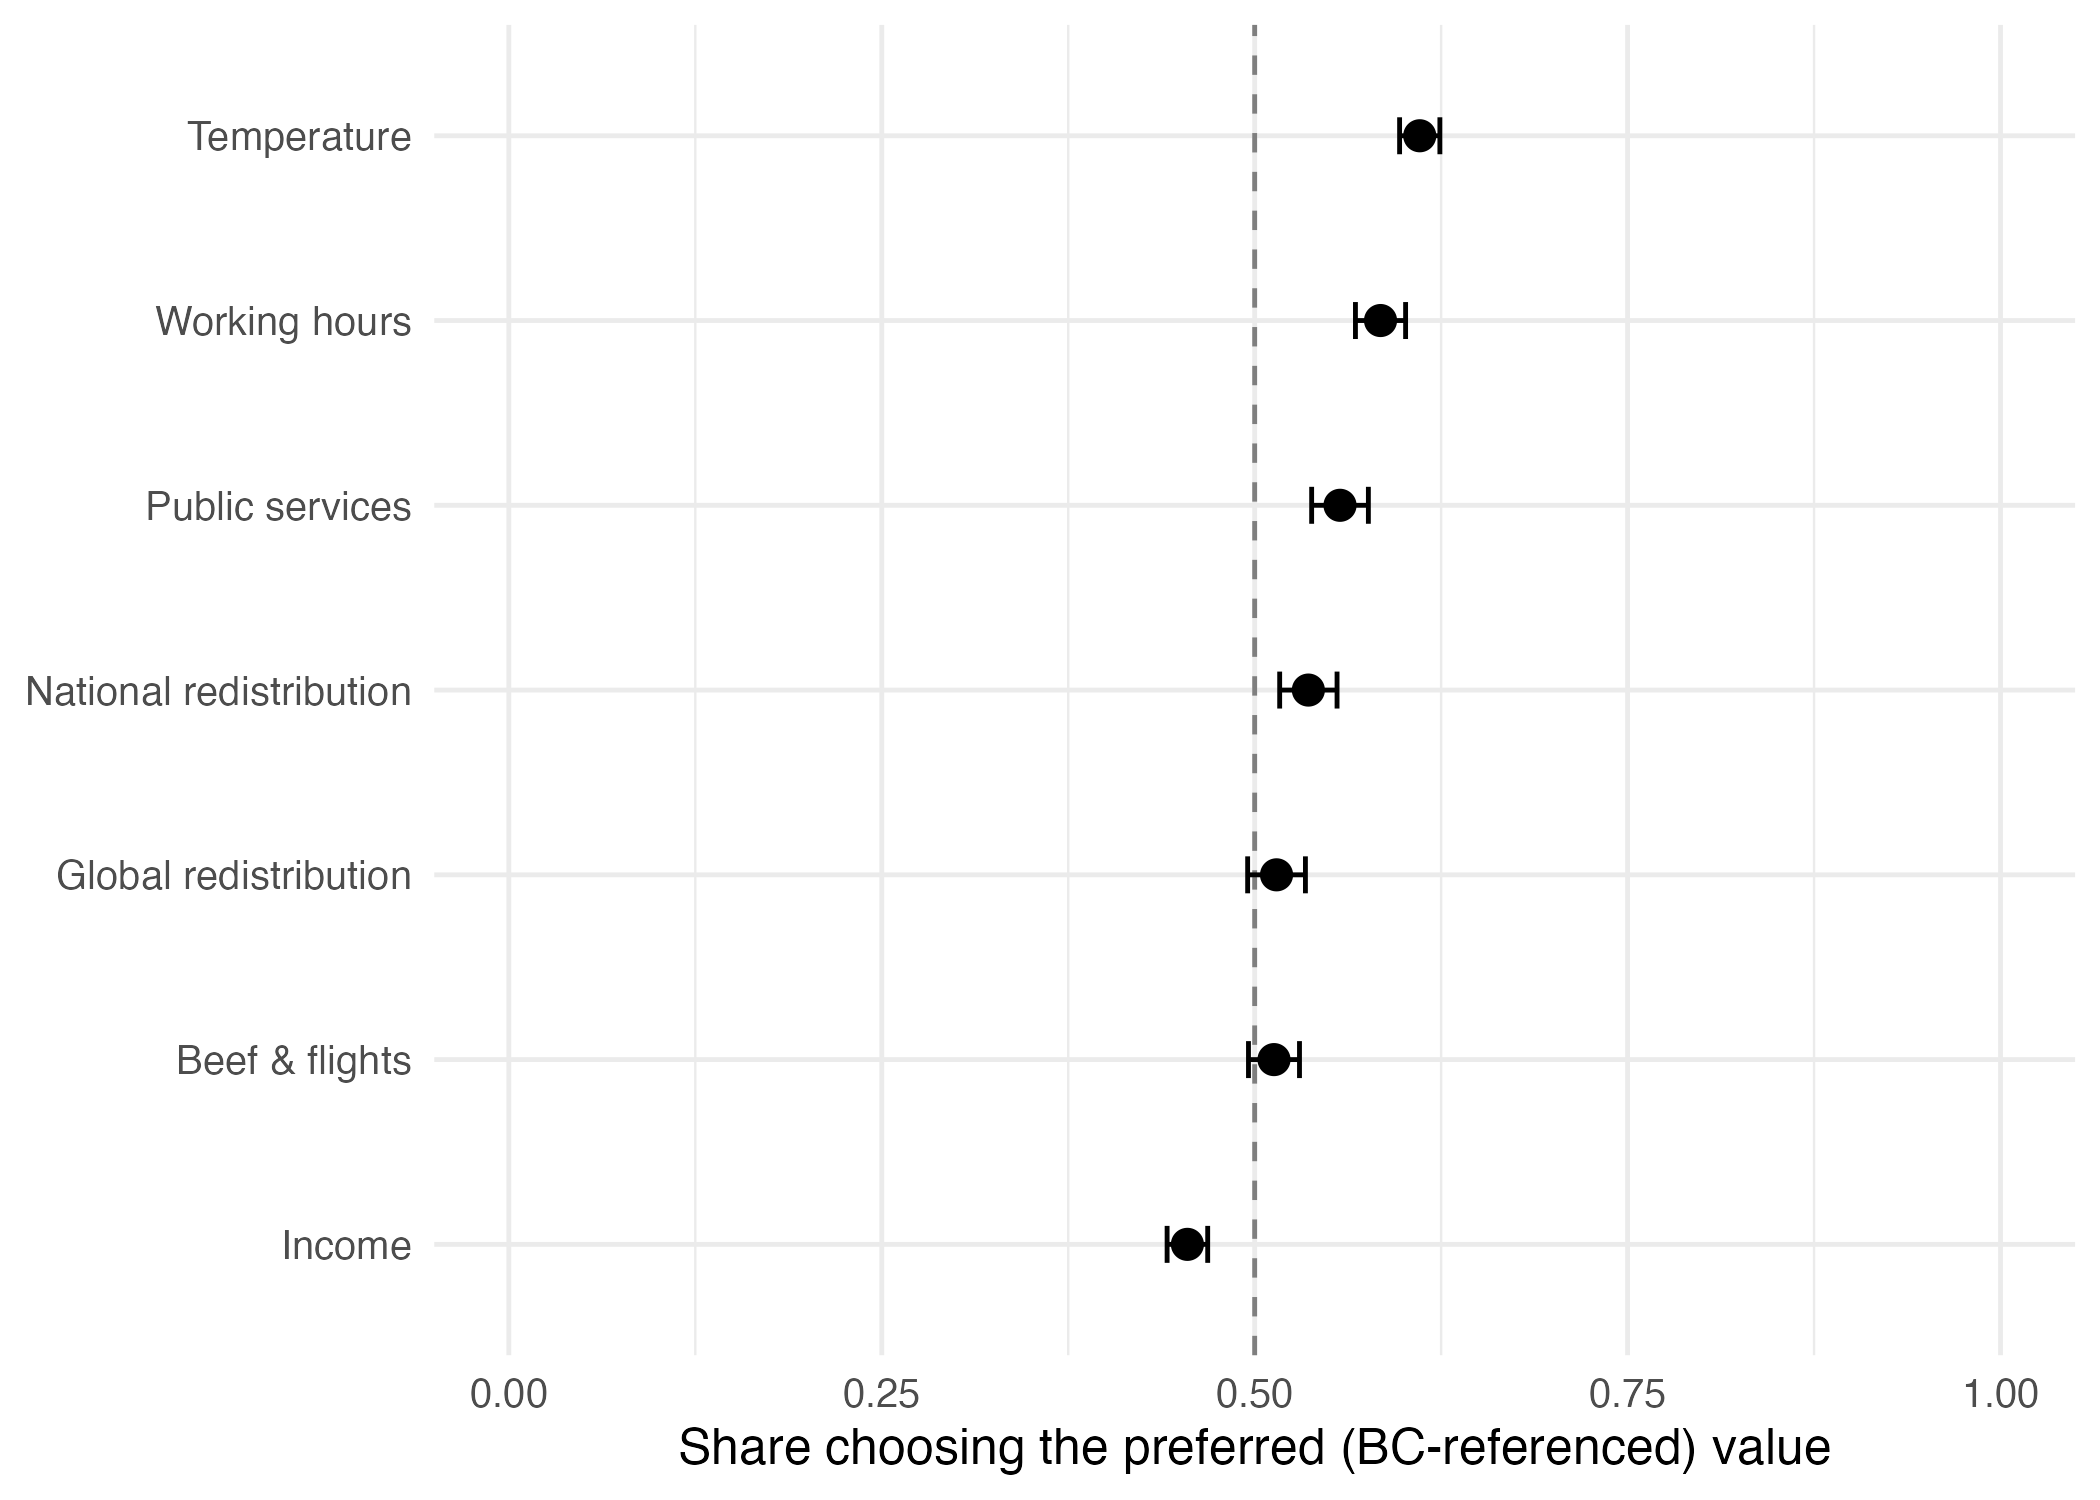
\includegraphics[width=0.8\textwidth]{fig1_share_preferred_value.png}
\caption{Share of cases choosing the preferred (BC-referenced) value, per attribute. \small{\textit{``I don't know'' pairs excluded (no side is chosen under indifference).}}}
\end{figure}

\begin{figure}[ht]
\centering
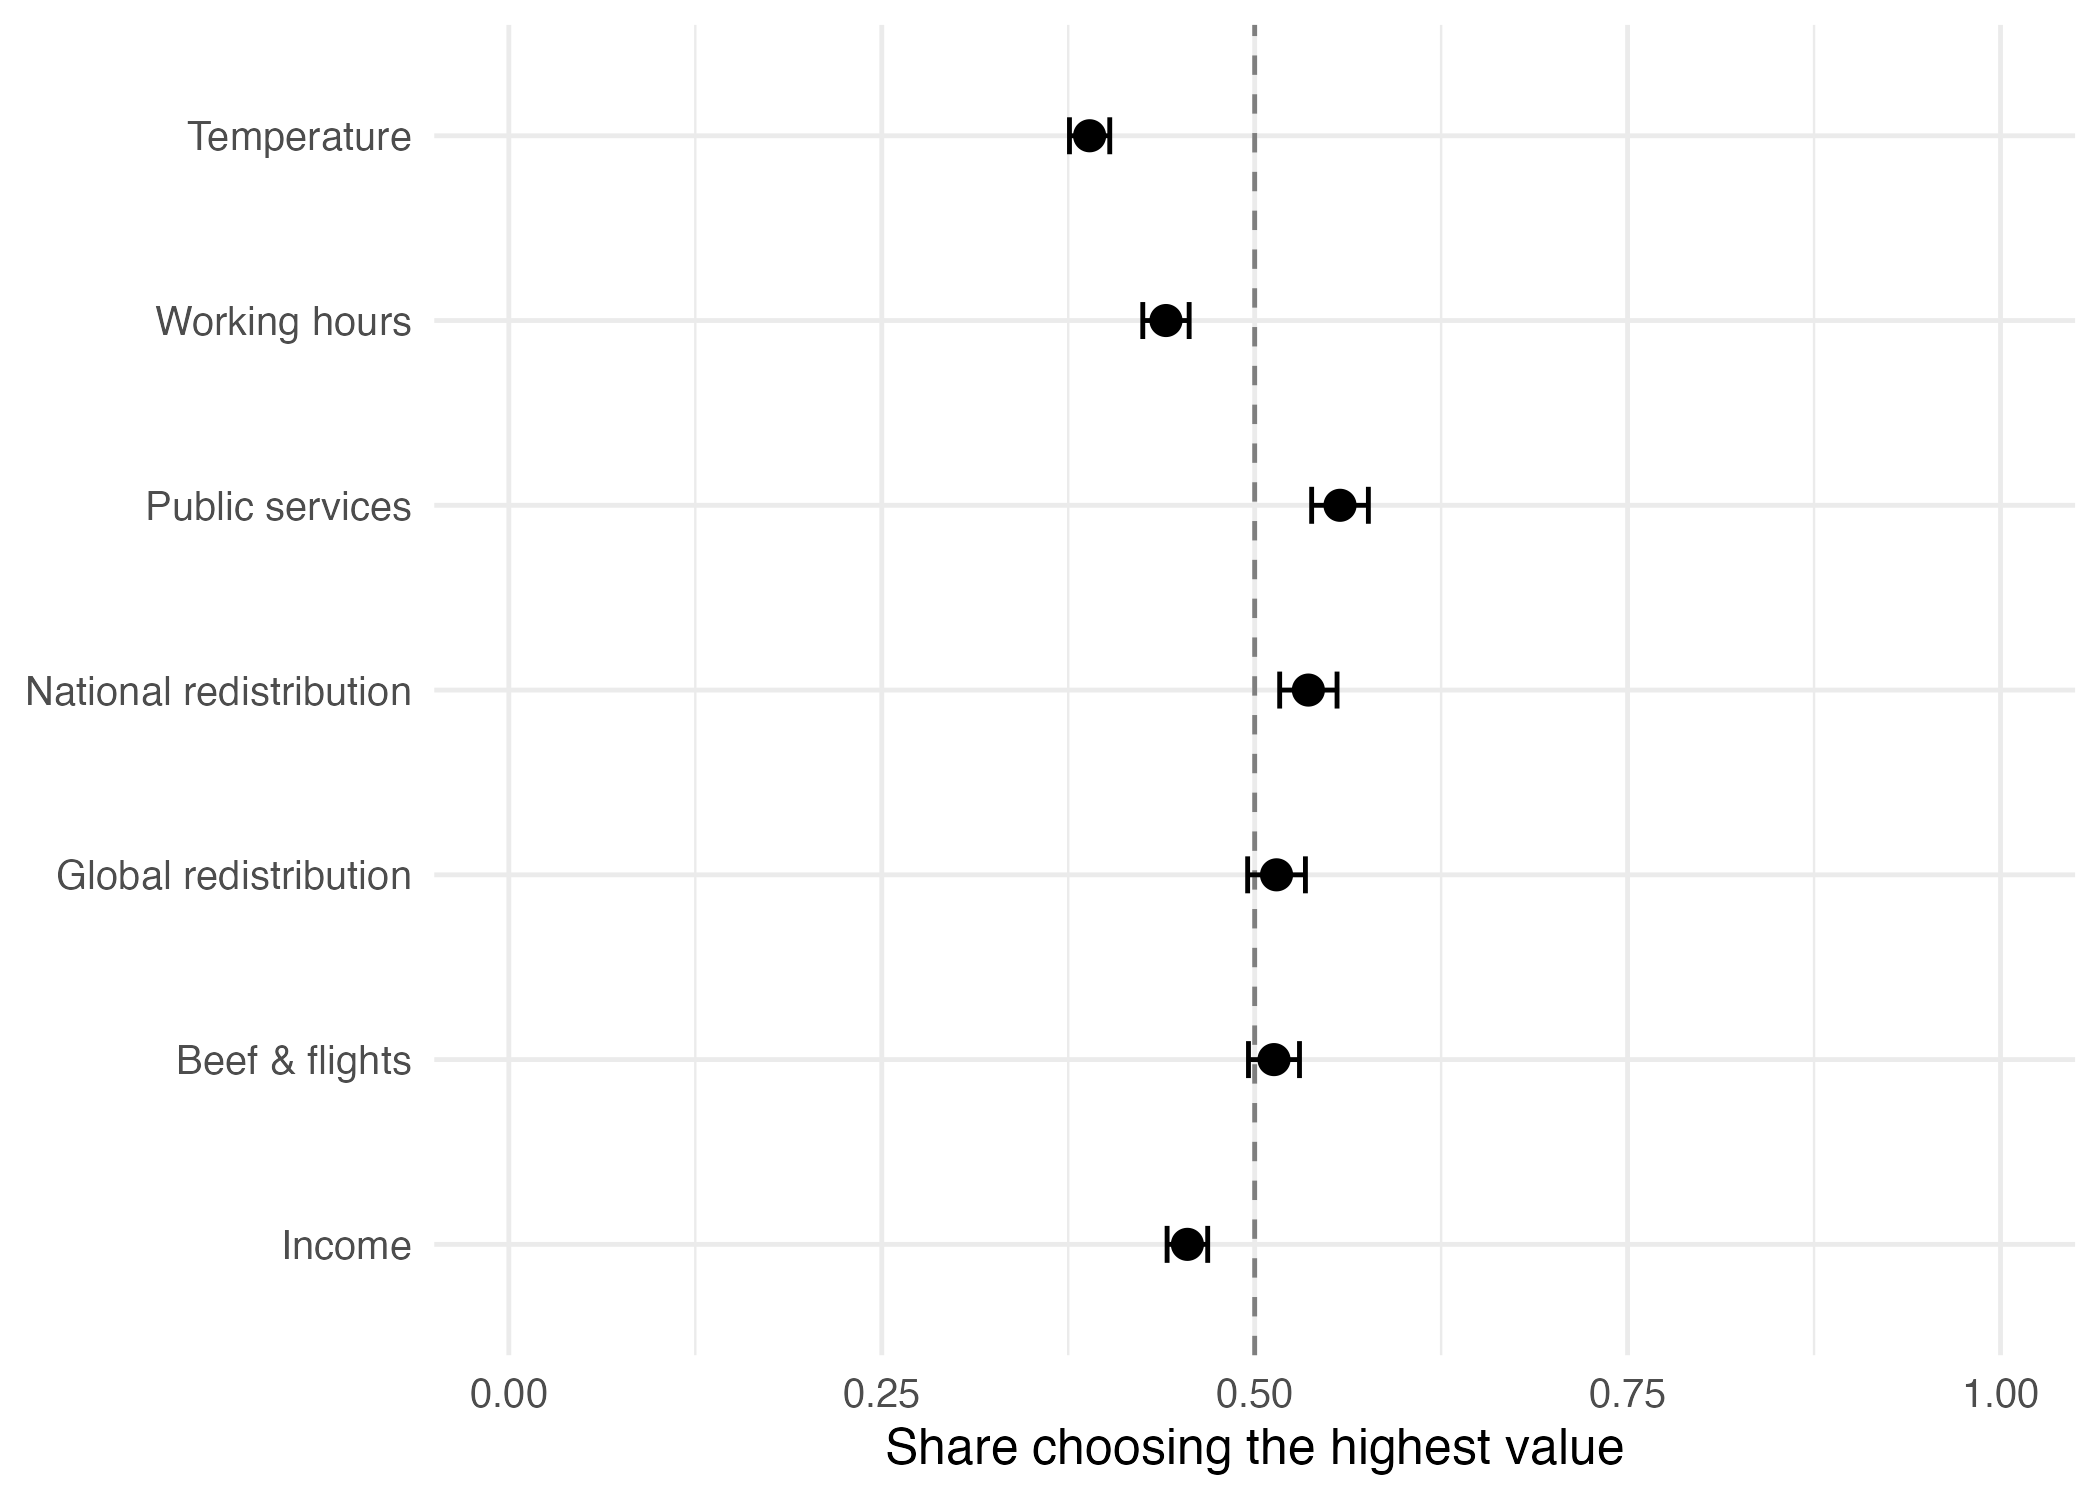
\includegraphics[width=0.8\textwidth]{fig1b_share_highest_value.png}
\caption{Supplementary: share of cases choosing the highest value, per attribute. \small{\textit{``I don't know'' pairs excluded.}}}
\end{figure}

\begin{figure}[ht]
\centering
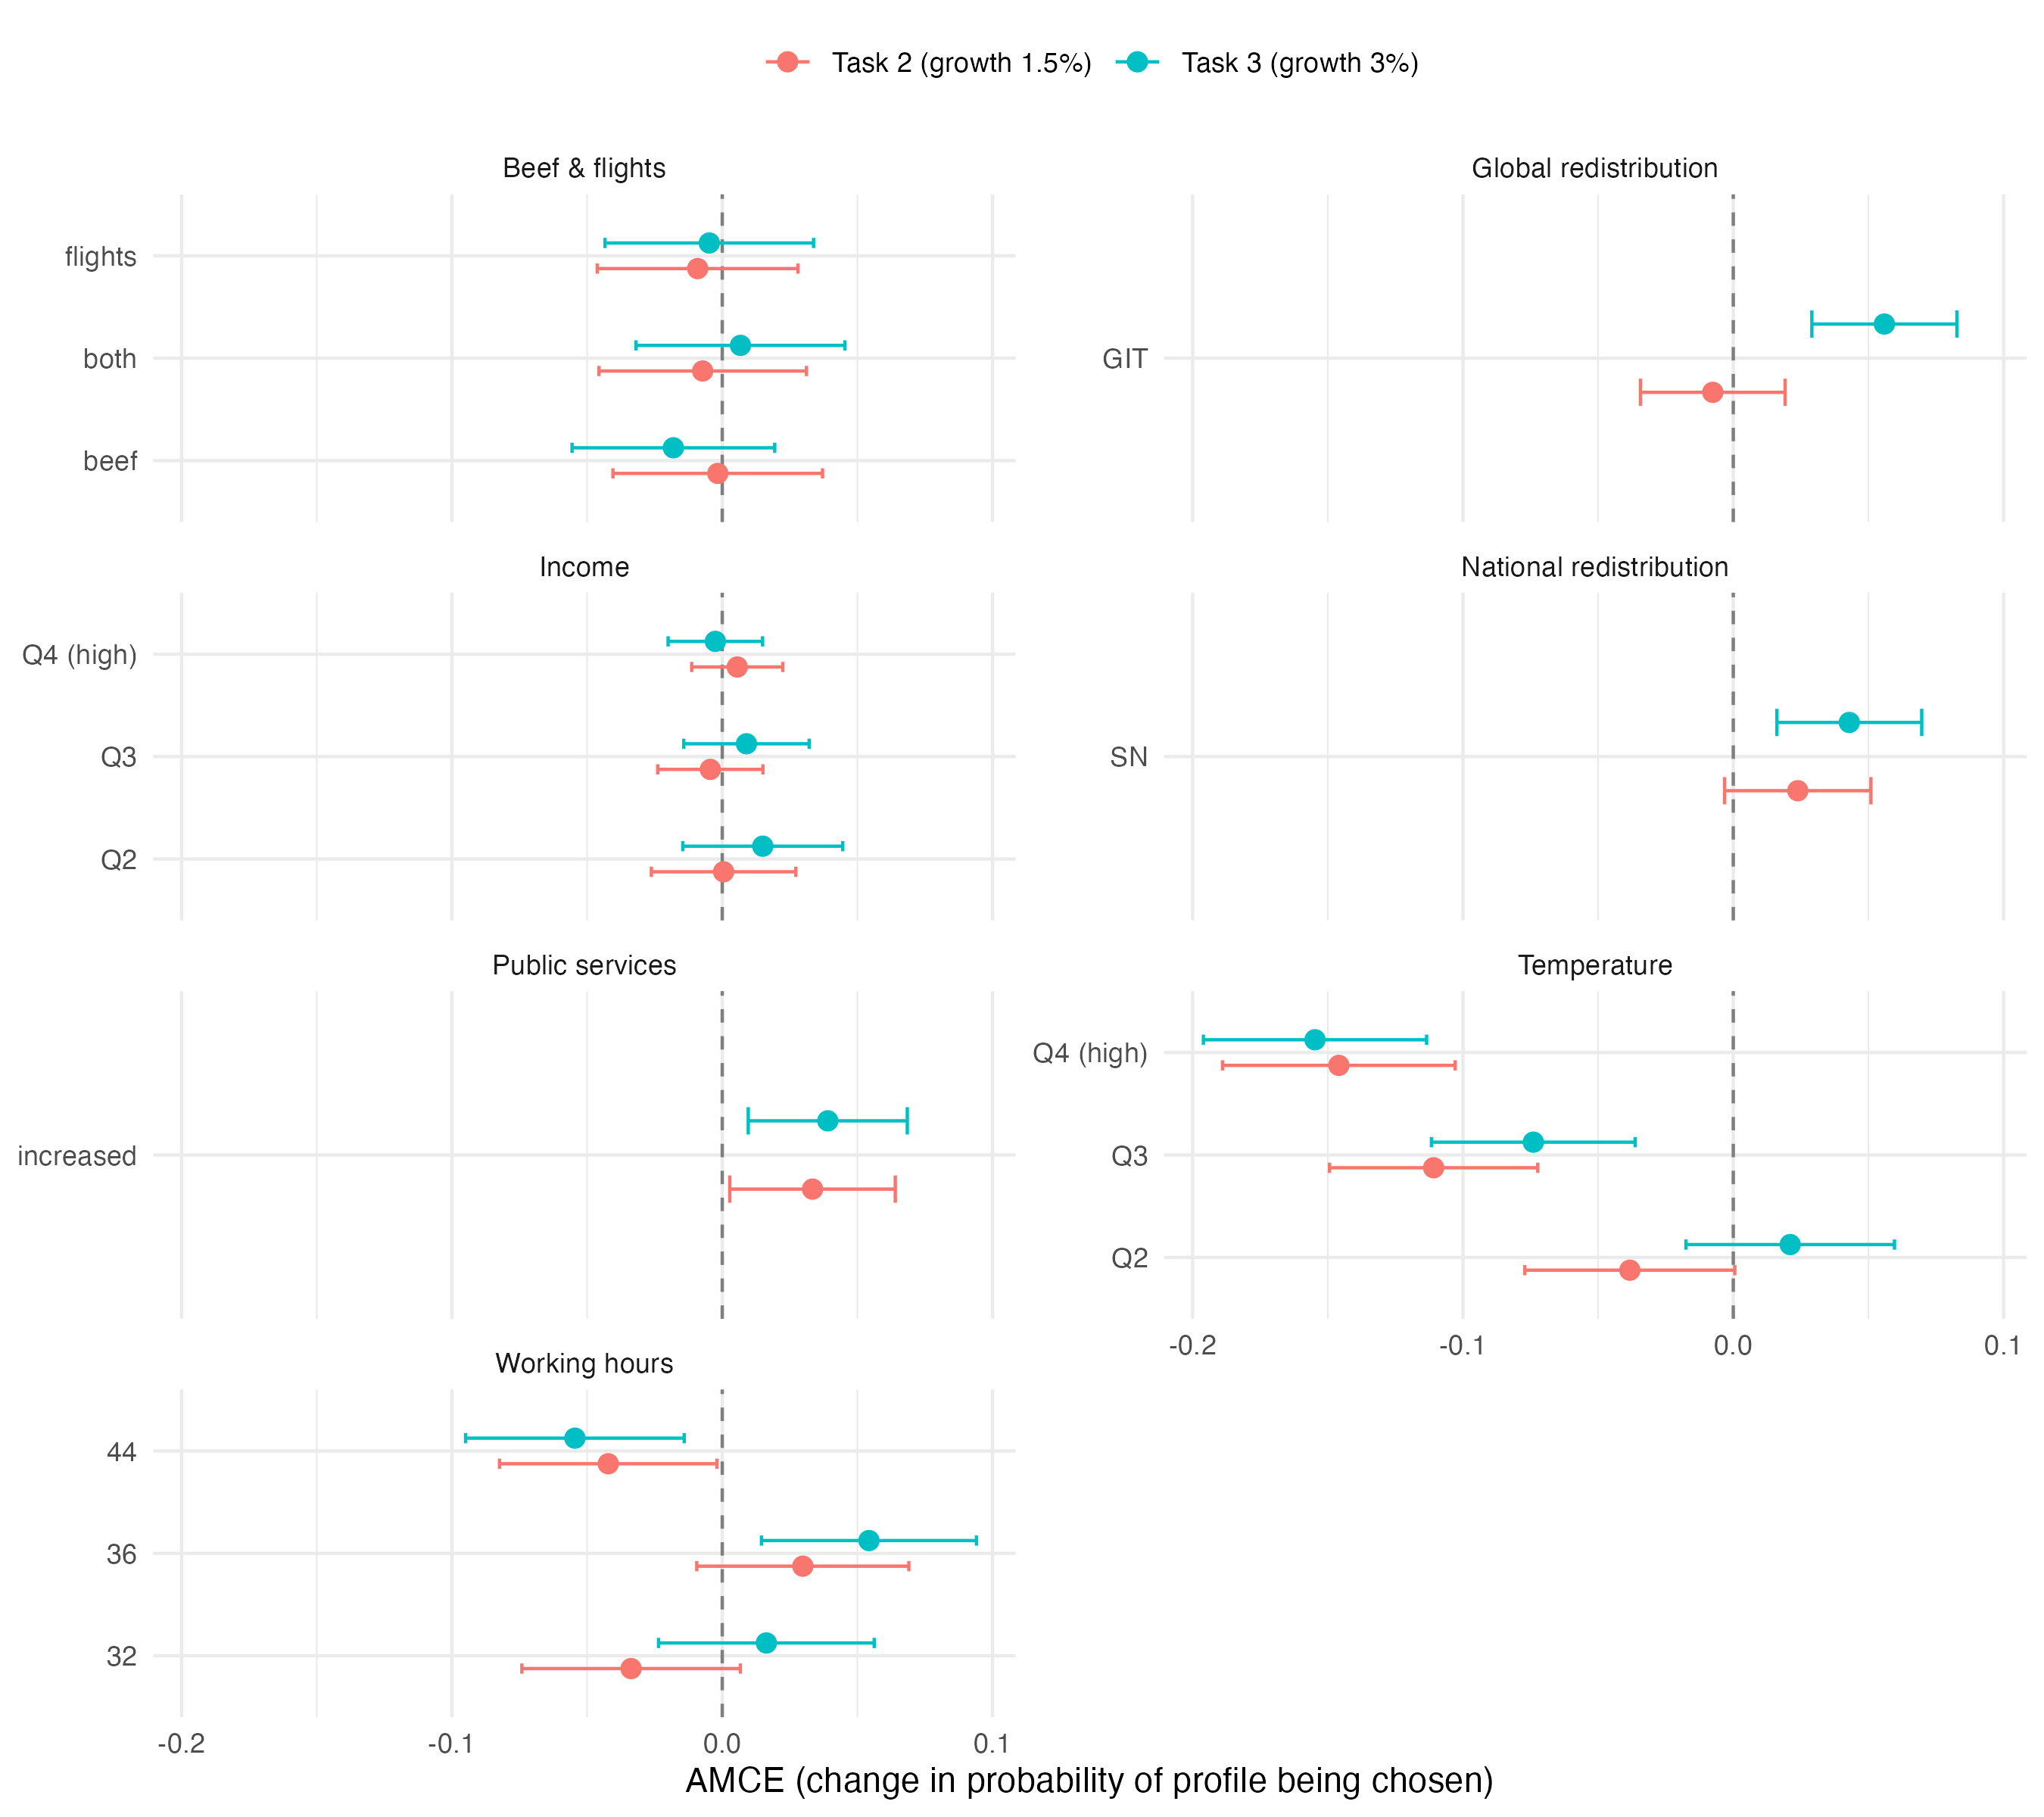
\includegraphics[width=0.9\textwidth]{fig2_amce_task2_vs_task3.png}
\caption{AMCEs for Task 2 and Task 3 (temperature/income binned into quartiles), superimposed. \small{\textit{``I don't know'' pairs excluded (\texttt{cjoint::amce()} requires a strict 0/1 matched pair).}}}
\end{figure}

\begin{figure}[ht]
\centering
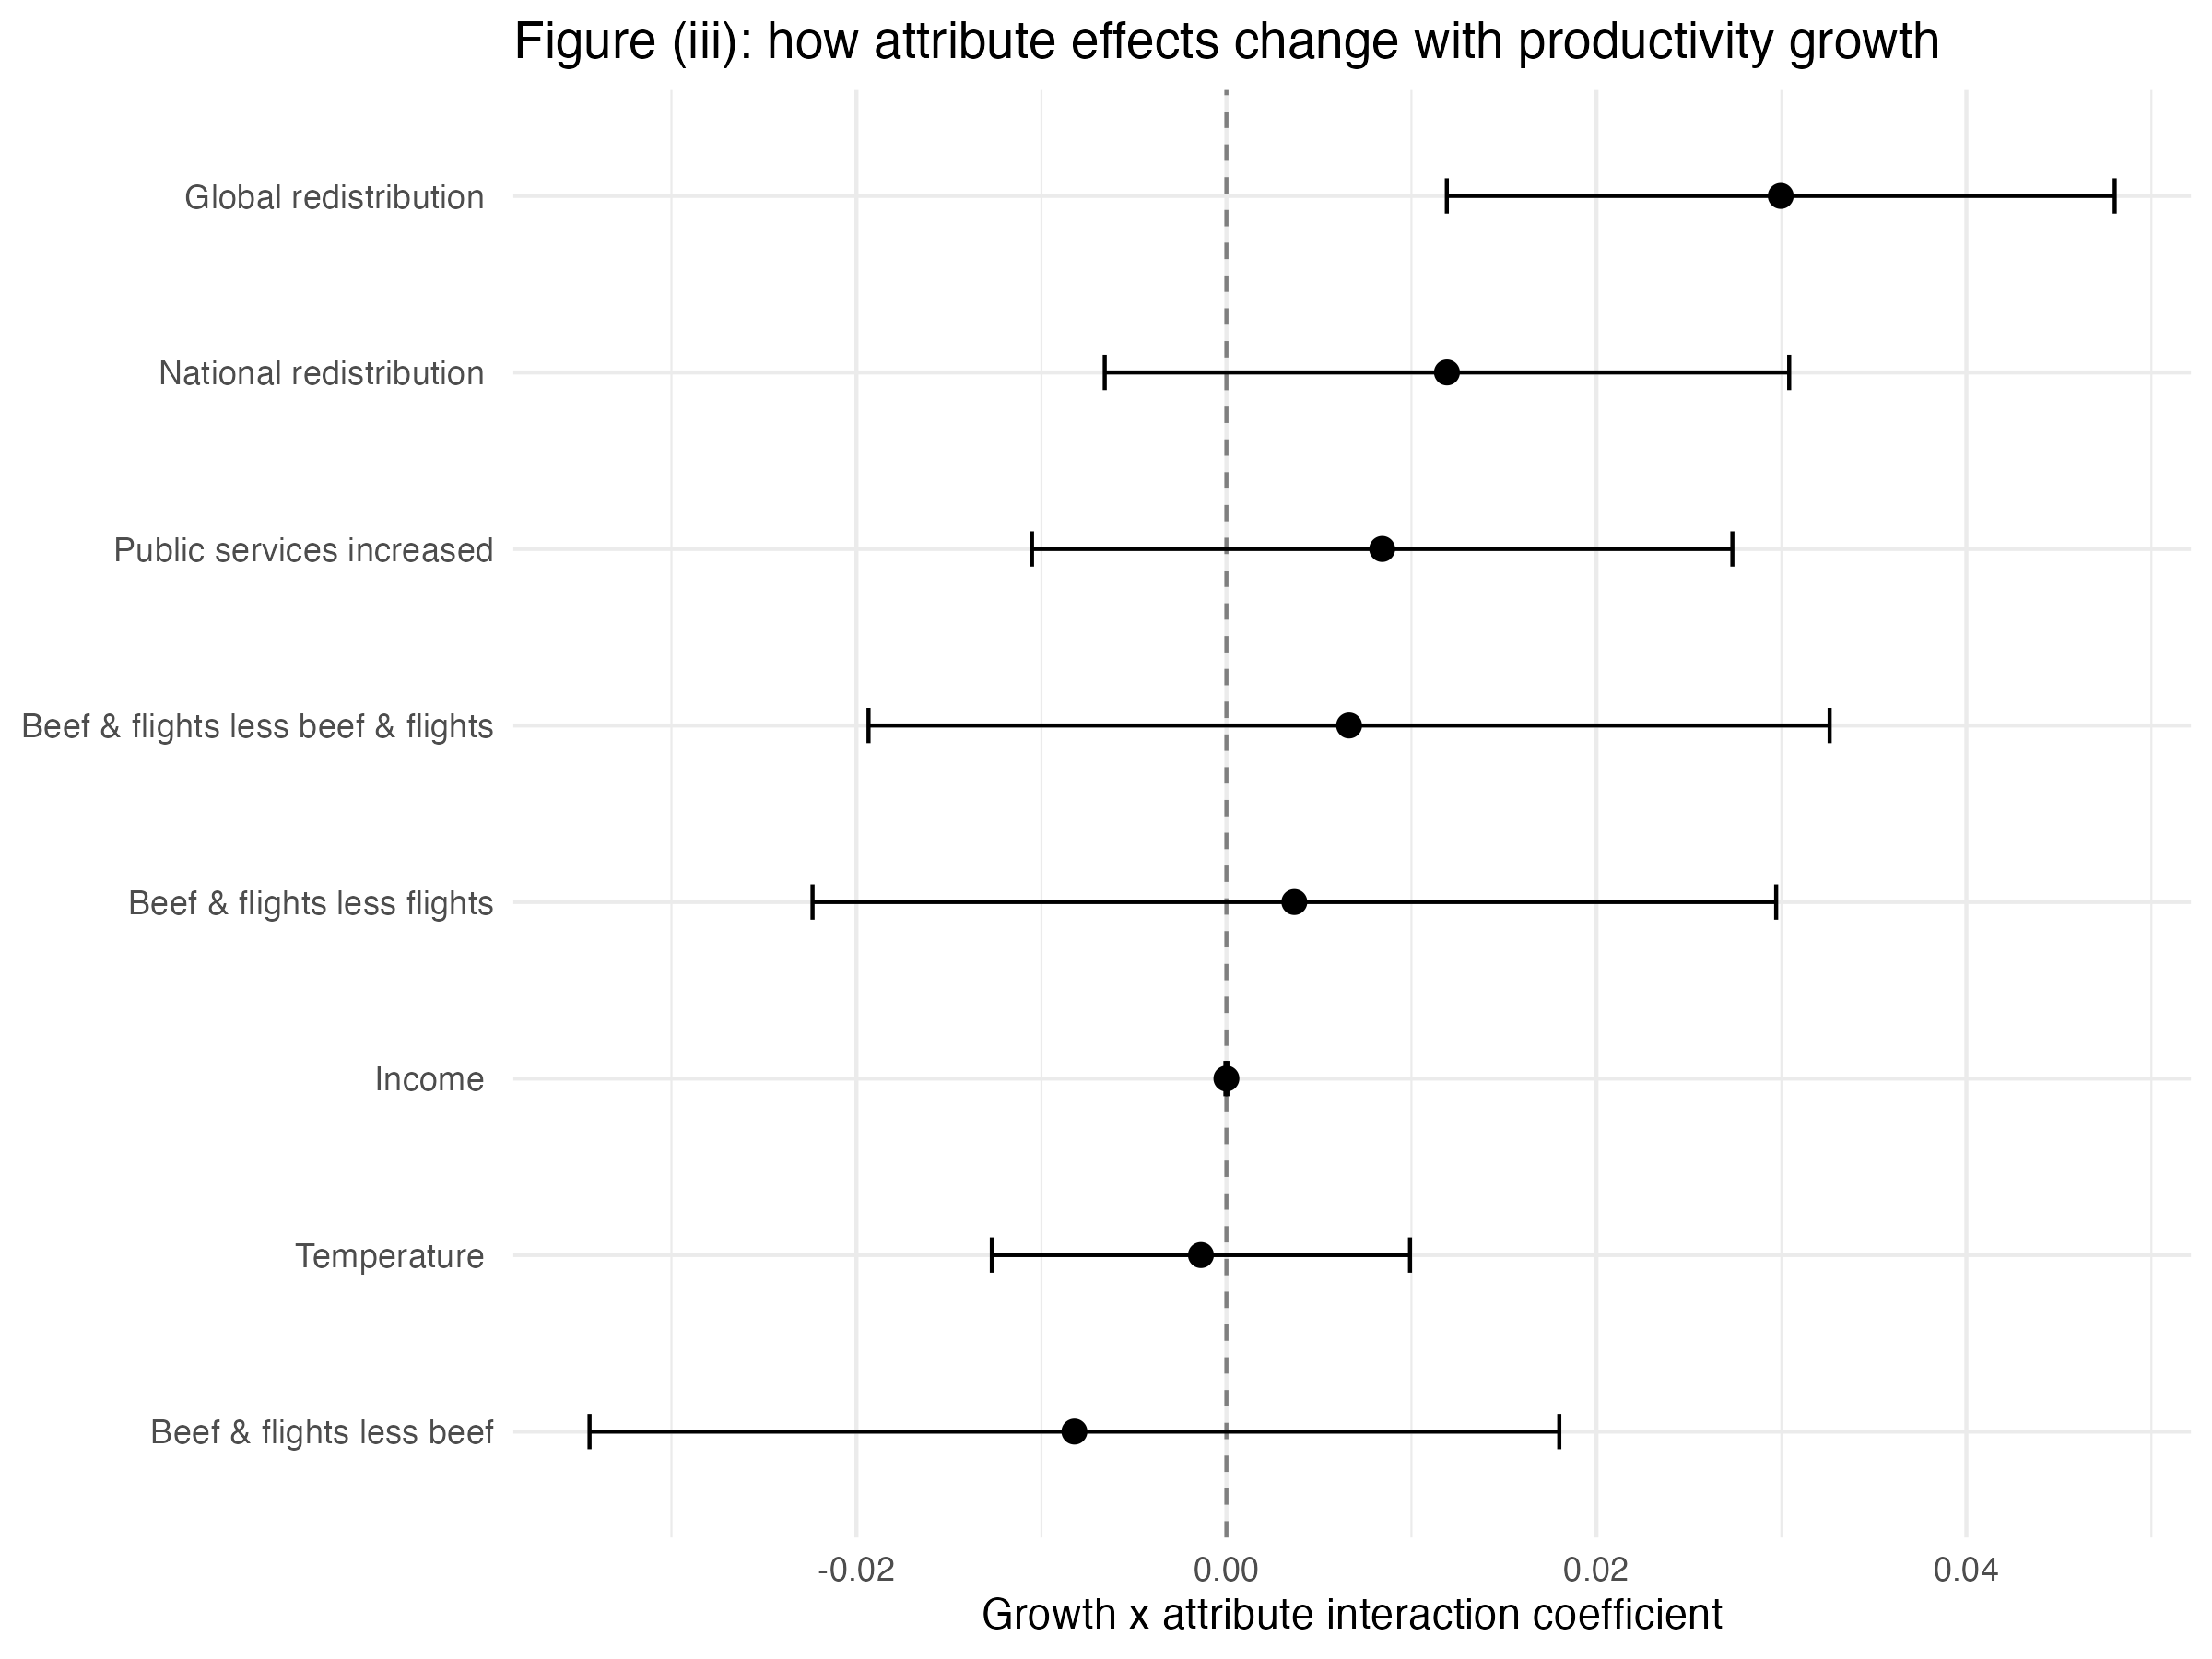
\includegraphics[width=0.8\textwidth]{fig3_growth_interactions.png}
\caption{Growth $\times$ attribute interaction coefficients, primary specification.}
\end{figure}

\begin{figure}[ht]
\centering
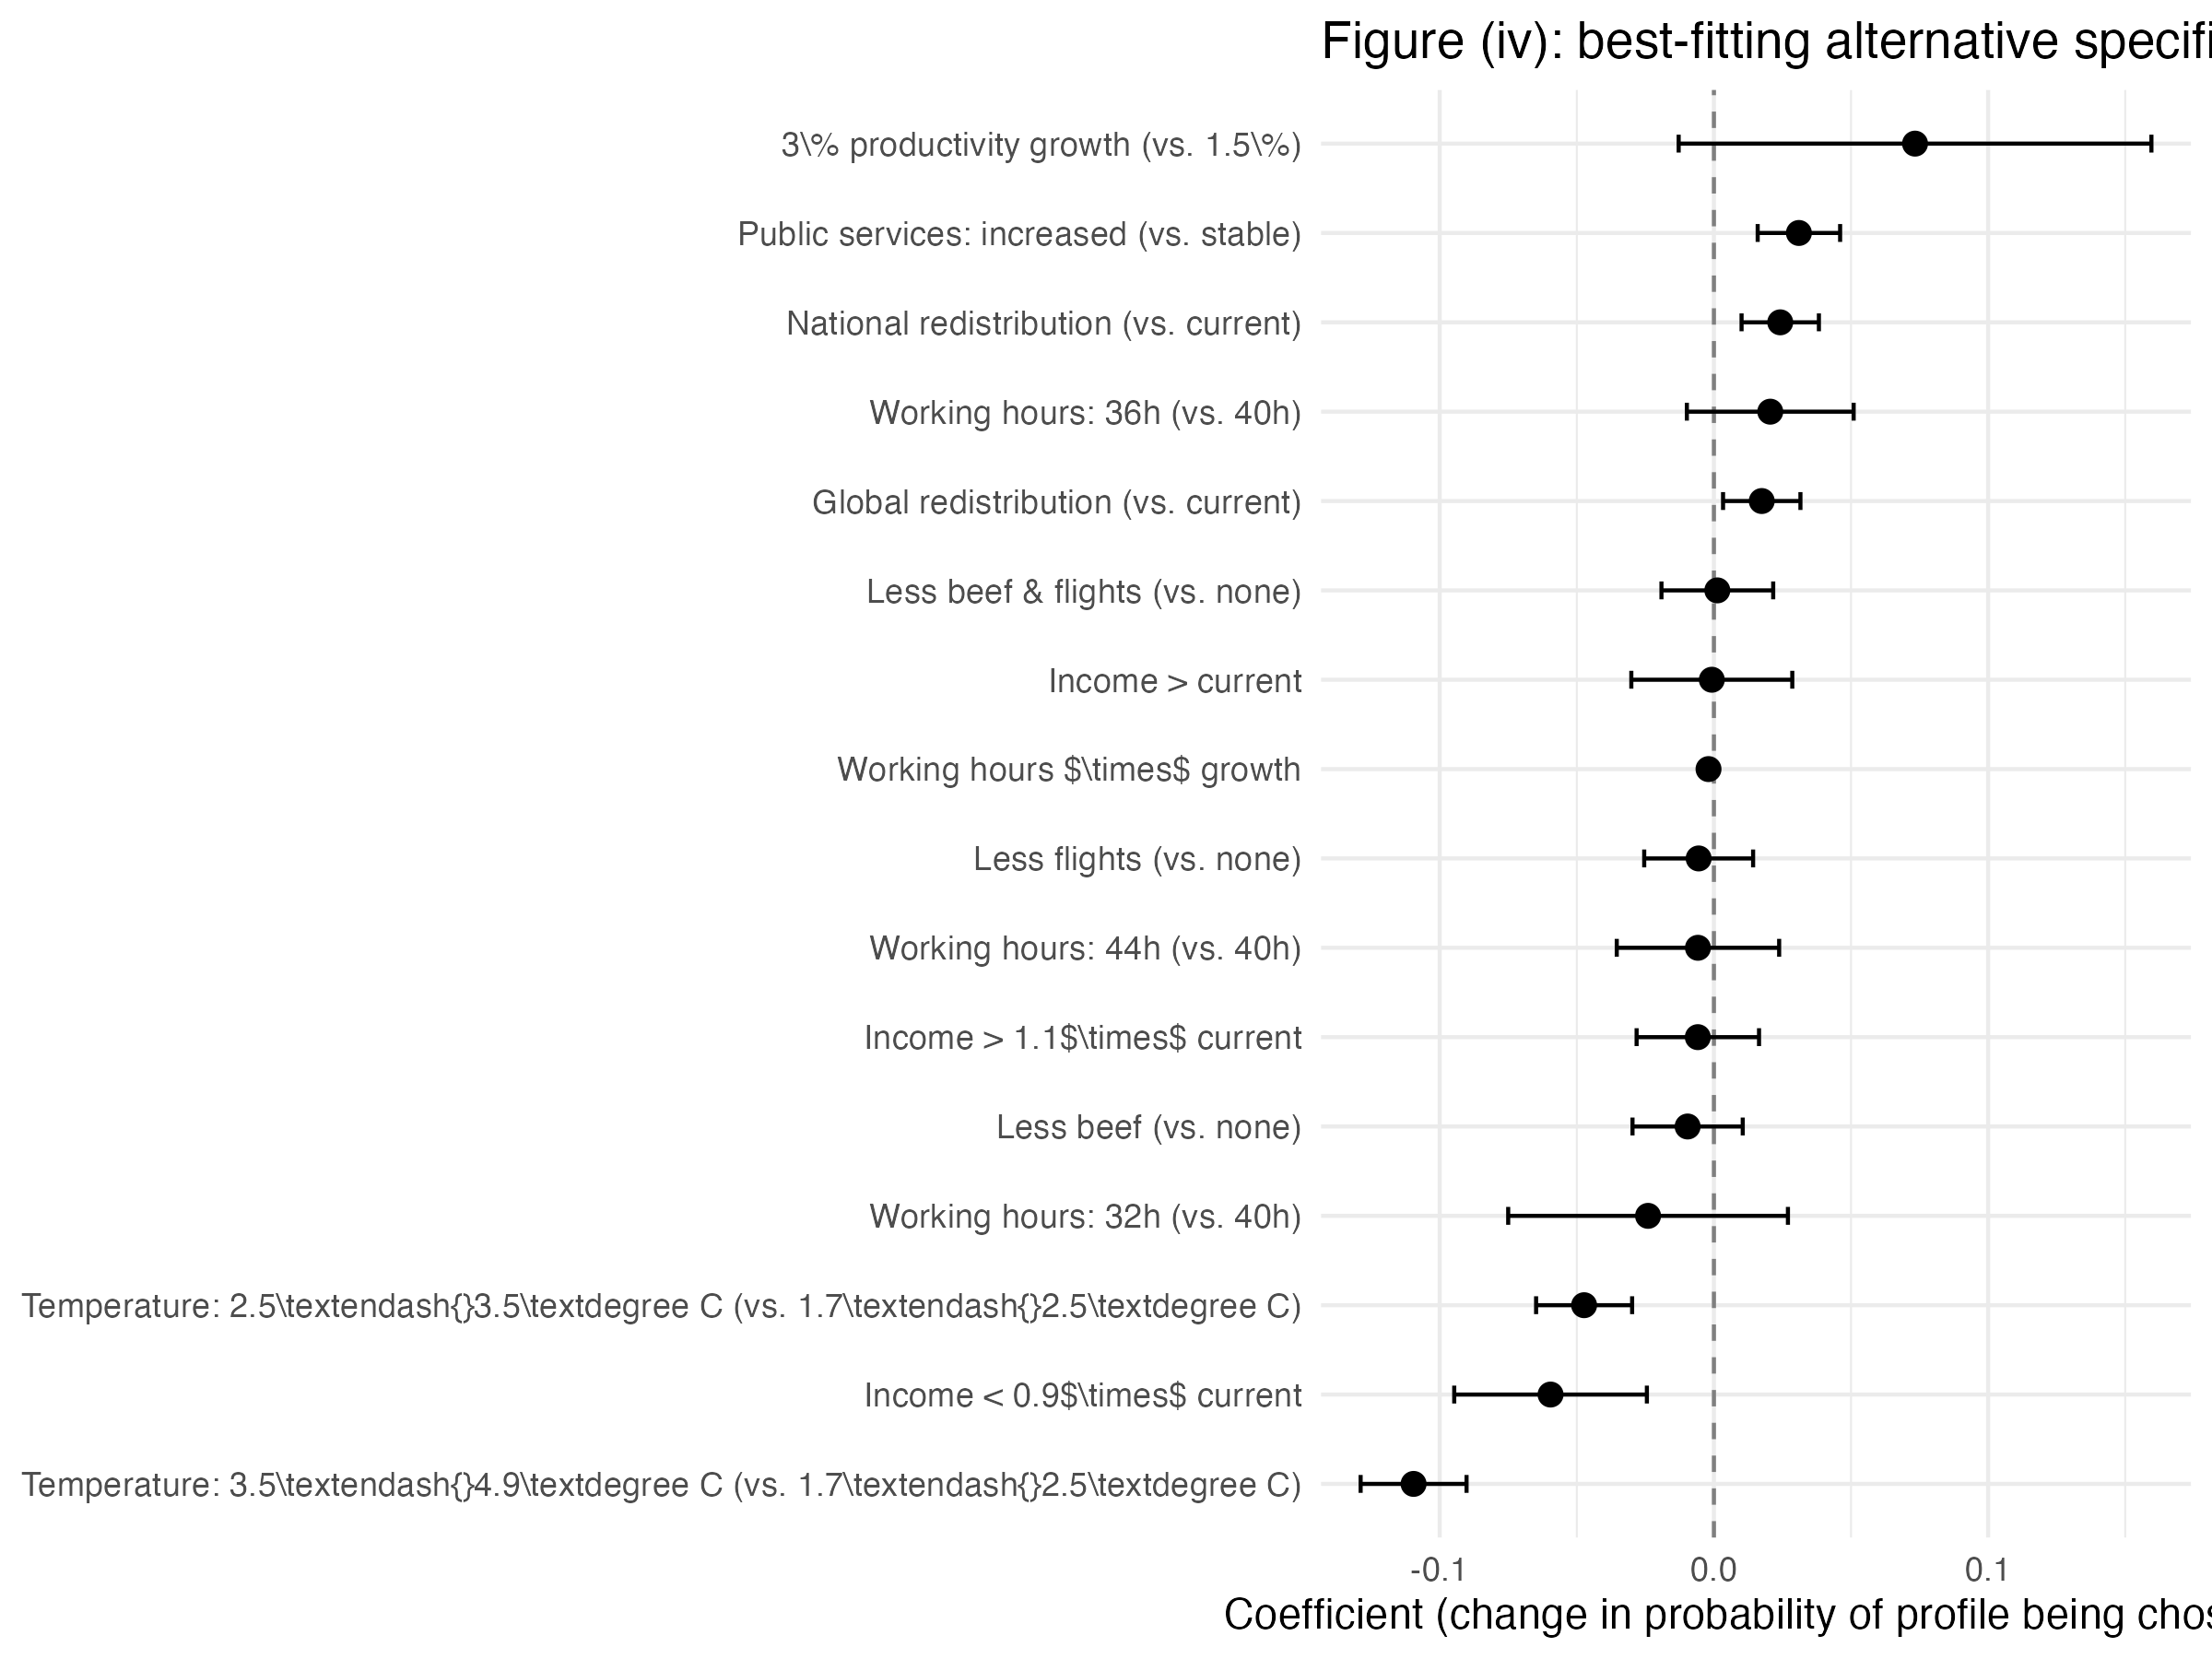
\includegraphics[width=0.8\textwidth]{fig4_secondary_spec.png}
\caption{Coefficients of the best-fitting (highest adjusted R\textsuperscript{2}) secondary specification.}
\end{figure}

\section{IDK}

\begin{table}[H]
    \centering
    \caption{Frequency of ``I don't know'' responses.}
    \begin{tabular}{ l c c c c }
\hline \hline
Task & N & N (IDK) & estimate & se \\
\hline
\hspace{0.05cm} Task 1 (FEW) & 3,247 & 1,038 & 32.0\% & (0.8\%) \\
\hspace{0.05cm} Task 2 (ANY) & 3,247 &   878 & 27.0\% & (0.8\%) \\
\hspace{0.05cm} Task 3 (ANY2) & 3,247 &   893 & 27.5\% & (0.8\%) \\
\hspace{0.05cm} Any of the 3 tasks & 3,247 & 1,431 & 44.1\% & (0.9\%) \\
\hline \hline
\end{tabular}
\begin{tablenotes}
\small
\item \textit{Notes:} By task, and for any of the 3 tasks. SE in parentheses (normal approximation).
\end{tablenotes}
    \label{tab:table11}
\end{table}


\begin{table}[H]
    \centering
    \caption{Predictors of ``I don't know'' responses.}
    \begin{tabular}{ l c c }
\hline \hline
 & estimate & se \\
\hline
\hspace{0.05cm} Age: 35-54 (vs. 18-34) & 0.0397** & (0.0199) \\
\hspace{0.05cm} Age: 55+ (vs. 18-34) & 0.0474** & (0.0206) \\
\hspace{0.05cm} Gender: Male (vs. Female) & -0.0691*** & (0.0134) \\
\hspace{0.05cm} Region: Northeast (vs. Northwest) & -0.0060 & (0.0198) \\
\hspace{0.05cm} Region: Center (vs. Northwest) & -0.0039 & (0.0197) \\
\hspace{0.05cm} Region: South (vs. Northwest) & 0.0071 & (0.0185) \\
\hspace{0.05cm} Region: Islands (vs. Northwest) & -0.0001 & (0.0244) \\
\hspace{0.05cm} Education: Upper secondary (vs. Compulsory/lower) & -0.0414 & (0.0269) \\
\hspace{0.05cm} Education: Tertiary (vs. Compulsory/lower) & -0.0971*** & (0.0282) \\
\hspace{0.05cm} Task: 1/FEW (vs. Task 2/ANY) & 0.0493*** & (0.0075) \\
\hspace{0.05cm} Task: 3/ANY2 (vs. Task 2/ANY) & 0.0049 & (0.0070) \\
\hline
\hspace{0.05cm} Observations & \multicolumn{2}{c}{3,245} \\
\hspace{0.05cm} R-squared & \multicolumn{2}{c}{0.015} \\
\hline \hline
\end{tabular}
\begin{tablenotes}
\small
\item \textit{Notes:} Sociodemographic characteristics and task/scenario features. Pooled linear probability model across the 3 DCE tasks, cluster-robust respondent-level SE in parentheses. *** p$<$0.01, ** p$<$0.05, * p$<$0.1. Baselines: Age vs. 18-34; Gender vs. Female ("Other", N=4, excluded); Region vs. Northwest; Education vs. Compulsory/lower secondary; Task vs. Task 2 (ANY). Political orientation not yet available (placeholder pending wave 1 merge).
\end{tablenotes}
    \label{tab:table12}
\end{table}


\end{document}
